\section{Kundekontakt}

\subsection{Interviews}

\begin{frame}{Udførte Interview}
To interviews blev udført 

\begin{itemize}
\item 4. April, 2. sprint - to pædagoger fra Birken \\ Præcisering af gamle krav
\item 8. Maj, 4. sprint - talepædagog \\Feedback fra oprindelig kontaktperson på Cars 
\end{itemize}

\end{frame}

\begin{frame}{Metode}
\begin{itemize}
\item Semistruktureret interview 
\item Åbne spørgsmål - tillader de interviewede at komme med idéer og feedback
\item Sætter en samtale igang om tilstanden af applikationen
\end{itemize}
\end{frame}

\begin{frame}{Resultat}
\begin{itemize}
\item Præcisering af krav
\item Nye krav
\item Feedback på produktet
\end{itemize}
\end{frame}

\begin{frame}{Problemstillinger}
\begin{itemize}
\item Interview timing
\begin{itemize}
\item Forkert email
\item Det vigtigste interview kom meget sent
\end{itemize}
\item Kunder skifter mening
\begin{itemize}
\item Forskellige kunder har forskellige meninger
\item Ændrer mening når implementation vises
\end{itemize}
\end{itemize}
\end{frame}

\subsection{Kravstyring}


\begin{frame}{Fælleskrav}
Der blev i fælleskab vedtaget krav fælles for alle projekter
\begin{itemize}
\item Uformelle 
\item Svære at holde styr på
\end{itemize}

Eksempler:
\begin{itemize}
\item GUI
\item Navne på projekter
\item Profilvælger
\end{itemize}
\end{frame}

\begin{frame}{Opdatering af krav}
\begin{itemize}
\item Baseret på udførte interviews
\item Userstories, tasks
\end{itemize}

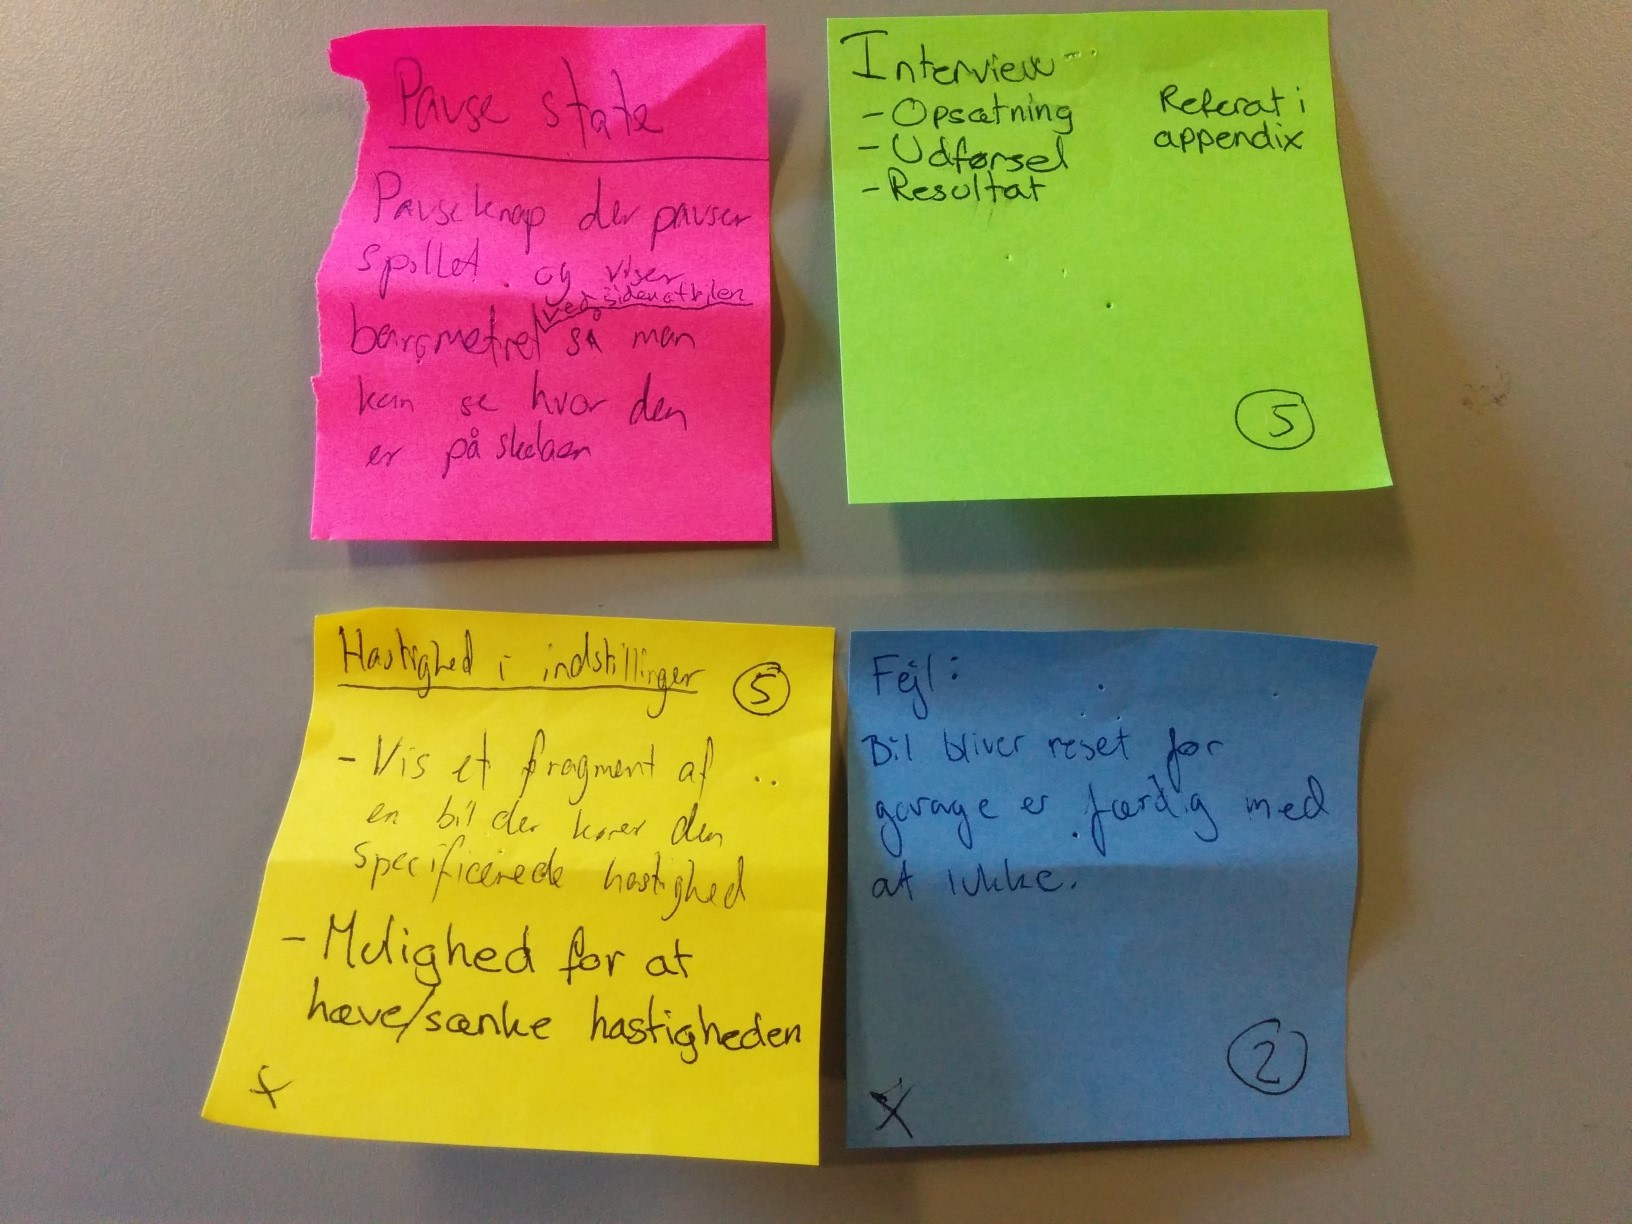
\includegraphics[width = 0.7\textwidth]{pgraphics/tasks}
\end{frame}

\begin{frame}{Eksempel}
Fra original Cars rapport
\begin{itemize}
\item \textit{It must be possible for the user to change the difficulty of the game}
\end{itemize}

Efter første interview
\begin{itemize}
\item \textit{Speed is alterable. The speed level is represented as a digit between 0 and 10.}
\item \textit{The placement and number of obstacles is alterable}
%\item The placement of obstacles should be in such a way, that it is possible to adapt it to both citizen with tendency to speaking too loud as well as those speaking too low.
\item\textit{ It should be possible, in settings, to switch\\ between avoiding objects and picking objects up.}
\end{itemize}
\end{frame}
